\let\negmedspace\undefined
\let\negthickspace\undefined
\documentclass[journal]{IEEEtran}


\setlength{\headheight}{1cm} % Set the height of the header box
\setlength{\headsep}{0mm}     % Set the distance between the header box and the top of the text
 \usepackage[a4paper,margin=10mm, onecolumn]{geometry}
\usepackage{gvv-book}
\usepackage{gvv}
\usepackage{cite}
\usepackage{amsmath,amssymb,amsfonts,amsthm}
\usepackage{algorithmic}
\usepackage{graphicx}
\usepackage{textcomp}
\usepackage{xcolor}
\usepackage{txfonts}
\usepackage{listings}
\usepackage{enumitem}
\usepackage{mathtools}
\usepackage{gensymb}
\usepackage{comment}
\usepackage[breaklinks=true]{hyperref}
\usepackage{tkz-euclide} 
\usepackage{listings}                                       
\def\inputGnumericTable{}                                
\usepackage[latin1]{inputenc}                                
\usepackage{color}                                            
\usepackage{array}                                            
\usepackage{longtable}                                       
\usepackage{calc}                                             
\usepackage{multirow}                                         
\usepackage{hhline}                                           
\usepackage{ifthen}                                           
\usepackage{lscape}
\usepackage{circuitikz}
\tikzstyle{block} = [rectangle, draw, fill=blue!20, 
    text width=4em, text centered, rounded corners, minimum height=3em]
\tikzstyle{sum} = [draw, fill=blue!10, circle, minimum size=1cm, node distance=1.5cm]
\tikzstyle{input} = [coordinate]
\tikzstyle{output} = [coordinate]

\begin{document}

\bibliographystyle{IEEEtran}
\vspace{3cm}

\title{1.11.15}
\author{AI25BTECH11013-Gautham}
 \maketitle
% \newpage
% \bigskip
{\let\newpage\relax\maketitle}

\renewcommand{\thefigure}{\theenumi}
\renewcommand{\thetable}{\theenumi}
\setlength{\intextsep}{10pt} % Space between text and floats


\numberwithin{equation}{enumi}
\numberwithin{figure}{enumi}
\renewcommand{\thetable}{\theenumi}                          
\textbf{Question}:\\
Write the direction ratios of the vector 3$\Vec{a}+2\Vec{b}$ where $\Vec{a}=\overrightarrow{i}+\overrightarrow{j}-2\overrightarrow{k}$ and $\Vec{b}=2\overrightarrow{i}-4\overrightarrow{j}+5\overrightarrow{k}$.\\
\solution \\
The given vectors $\Vec{a}$ and $\Vec{b}$ are 
\begin{align}
\Vec{a}=\myvec{1 \\ 1 \\ -2} \\
\Vec{b}=\myvec{2 \\ -4 \\ 5}
\end{align}
The direction ratios of the vector $3\Vec{a}+2\Vec{b}$ are
\begin{align}
  3\Vec{a}+2\Vec{b}=\myvec{a&b}\myvec{3 \\ 2}\\
  3\Vec{a}+2\Vec{b}=\myvec{1 & 2 \\ 1 &-4 \\ -2 & 5}\myvec{3\\2}\\
  3\Vec{a}+2\Vec{b}=\myvec{3(1)+2(2)\\3(1)+2(-4)\\3(-2)+2(5)}\\
  3\Vec{a}+2\Vec{b}=\myvec{7\\-5\\4}
\end{align}
\begin{figure}[ht]
    \centering
    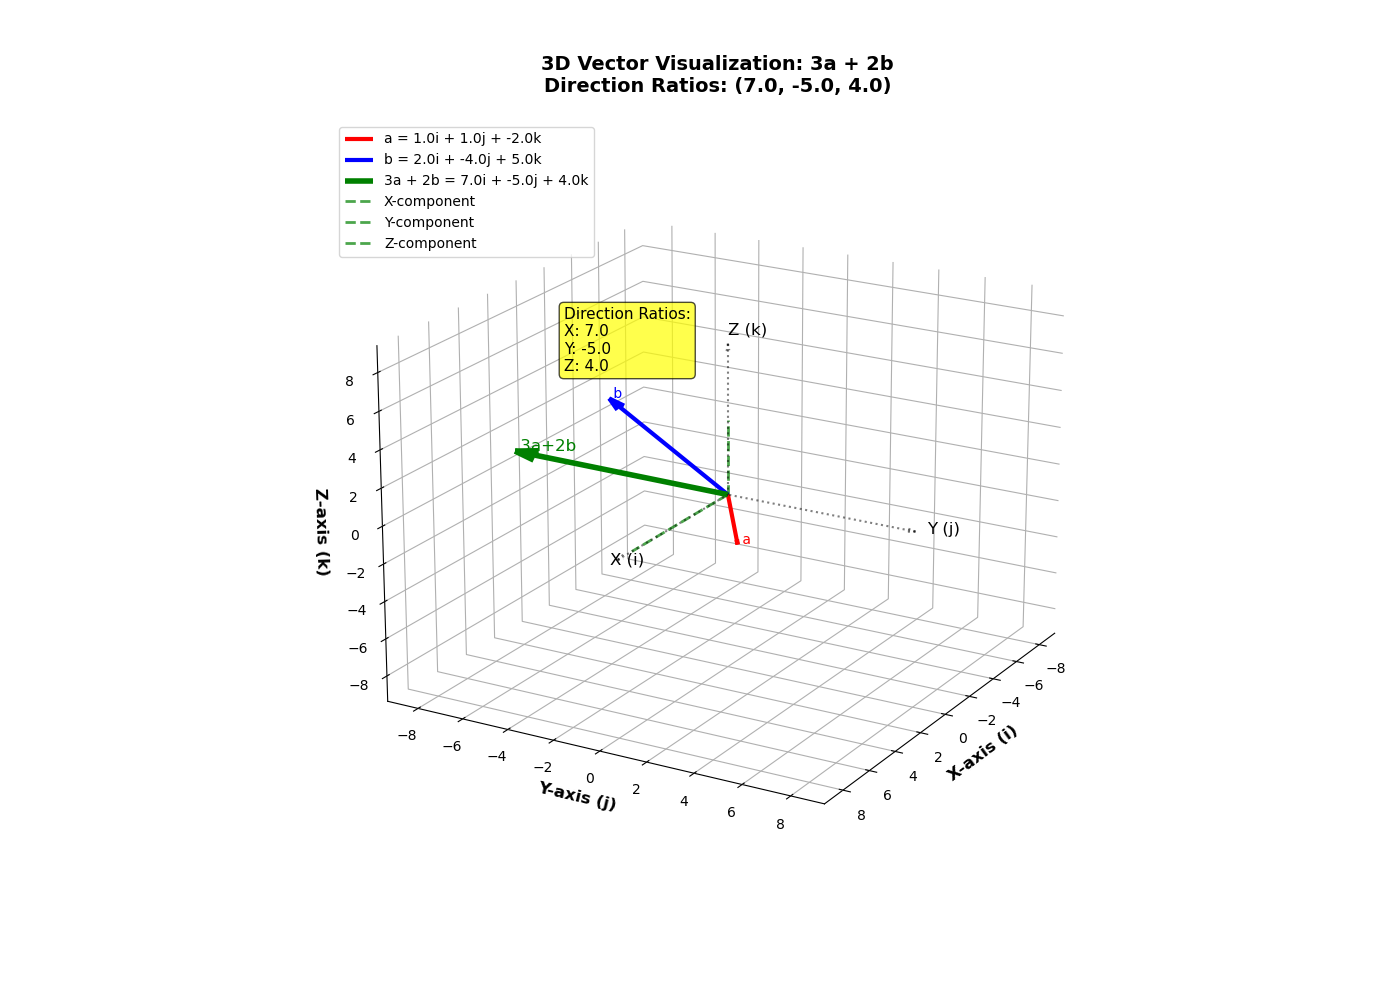
\includegraphics[height=0.6\textheight, keepaspectratio]{figs/fig1.png}
    \label{figure_1}
\end{figure}

\end{document}
